% !TEX root = ../main.tex
% 本文件由 build-tex.sh 从 29-DSP指南-第29章中译.md 生成，改内容请改 md 后重新生成

\chapter{DSP 入门}\label{ch-29}

一旦你确定数字信号处理器(Digital Signal
Processor)适合你的应用，就需要一个入门的途径。许多厂商会以低价卖给你一套评估套件(evaluation
kit)，让你亲手体验他们的产品。这是很好的学习工具：不管你是新手还是老手，它都是熟悉某款
DSP 的最好方式。例如，Analog Devices 公司提供 EZ-KIT®
Lite，向潜在客户介绍它的 SHARC® 系列数字信号处理器。只要 179
美元，你就能得到看 DSP
实际运行所需的全部硬件和软件。其中包括套件自带的''现成''程序，也包括你自己用汇编或
C 编写的应用程序。假设你从 Analog Devices
买了这样一套套件，玩了几天。本章概述你可能会看到和学到的东西。

\begin{quote}
原书脚注：SHARC、EZ-KIT、EZ-LAB、VisualDSP、EZ-ICE、SHARC 标志、Analog
Devices 标志和 VisualDSP 标志都是 Analog Devices, Inc.~的注册商标。
\end{quote}

\section{ADSP-2106x 系列}

上一章我们介绍了 ADSP-2106x ``SHARC''
系列数字信号处理器的一般工作原理。表 29-1
列出了这个系列的各个成员。这些器件使用同一种体系结构，但片上存储器(on-chip
memory)的容量不同，这是决定选用哪一款的关键因素。存储器访问是 DSP
系统中常见的瓶颈。SHARC DSP 的解决办法是提供充足的片上双端口
SRAM(dual-ported
SRAM)。不过，你最不想做的事，就是为用不上的存储器付钱。DSP
常常用在对成本敏感的产品里，比如手机和 CD
播放机。换句话说，这个系列的划分既由技术决定，也由市场决定。

这个系列中最老的成员是
ADSP-21020。这款芯片包含核心体系结构，但没有片上存储器，也不处理
I/O。这意味着它不能作为独立的计算机工作，需要外部元件才能构成一个能用的系统。其他器件都是单芯片上的完整计算机，只需要电源和某种把程序装进存储器的方式（比如外部
PROM 或数据链路）就能运行。

\textbf{表 29-1　SHARC 系列的成员。}

{\def\LTcaptype{none} % do not increment counter
\begin{longtable}[]{@{}
  >{\raggedright\arraybackslash}p{(\linewidth - 4\tabcolsep) * \real{0.3333}}
  >{\raggedright\arraybackslash}p{(\linewidth - 4\tabcolsep) * \real{0.3333}}
  >{\raggedright\arraybackslash}p{(\linewidth - 4\tabcolsep) * \real{0.3333}}@{}}
\toprule\noalign{}
\begin{minipage}[b]{\linewidth}\raggedright
产品
\end{minipage} & \begin{minipage}[b]{\linewidth}\raggedright
存储器
\end{minipage} & \begin{minipage}[b]{\linewidth}\raggedright
说明
\end{minipage} \\
\midrule\noalign{}
\endhead
\bottomrule\noalign{}
\endlastfoot
AD1460 & 4 Mbit × 4 & Quad-SHARC，四片 ADSP-21060 装在同一个模块里；在仅
2.05″×2.05″×0.16″ 的体积内提供惊人的 480 MFLOPS \\
ADSP-21160M & 4 Mbit &
新品！采用单指令多数据（SIMD）核心体系结构；为多处理做了优化，带链路口、64
位外部总线和 14 个 DMA 通道 \\
ADSP-21060 & 4 Mbit &
系列中的主力；存储器最多；带链路口，用于高速数据传输和多处理 \\
ADSP-21062 & 2 Mbit & 功能与 ADSP-21060
相同，但内部存储器（SRAM）较少，成本更低 \\
ADSP-21061 & 1 Mbit & EZ-KIT Lite
用的低成本版本；存储器较少、没有链路口；串口的 DMA 功能有所增强 \\
ADSP-21065L & 544 kbit & 系列的新成员；速度快、价格非常低（10
美元）。会把很多定点应用吸引到 SHARC 系列来 \\
ADSP-21020 & 无 & 系列中最老的成员。包含核心处理器，但没有片上存储器和
I/O 接口。算不上真正的 SHARC DSP \\
\end{longtable}
}

注意表 29-1 中，即使是低端产品也有相当可观的存储器。例如，ADSP-21065L 有
544 kbit 的内部 SRAM，足以存放 6～8 秒的数字化语音（每秒 8k
个采样，每个采样 8 位）。在系列的高端，ADSP-21060 有 4 Mbit
存储器，足以存下一整幅数字图像（512×512 像素，每像素 8
位）还绰绰有余。如果还需要更多存储器，任何一款器件都可以很容易地外接
SRAM（或更慢的存储器）。

除了存储器，这些系列成员在 I/O 部分也有区别。ADSP-21060 和
ADSP-21062（高端）各有六个链路口(link port)。这些是 4
位宽的并行连接，用于在多处理系统中把多片 DSP
组合起来，以及其他需要灵活高速 I/O 的应用。ADSP-21061 和
ADSP-21065L（低端）没有链路口，但有更多的 DMA
通道来协助串口工作。你还会看到这些型号后面带个 ``L'' 或 ``M''，比如
``ADSP-21060L''。这表示该器件的工作电压低于传统的 5.0
伏。例如，ADSP-21060L 工作在 3.3 伏，而 ADSP-21160M 只用 2.5 伏。

1998 年 6 月，Analog Devices 发布了第二代 SHARC 体系结构，推出了
ADSP-21160。它采用单指令多数据（Single Instruction Multiple
Data，SIMD，读作 ``sim-dee''）核心体系结构，工作频率 100
MHz，存储器总线带宽提高到每秒 1600 兆字节，有两条 64
位数据总线，以及四个用于定点计算的 80 位累加器。总的来说，新的
ADSP-21160M 只用 46 微秒就能完成一次 1024 点 FFT。SIMD DSP
包含第二套运算单元（算术逻辑单元、桶形移位器(barrel
shifter)、数据寄存器堆和乘法器），使 ADI 既能保持与 ADSP-2106x
系列的向后代码兼容，又提供了一条性能提升至多十倍的路线。

\section{SHARC EZ-KIT Lite}

EZ-KIT Lite 提供了学习 SHARC DSP
所需的一切，包括硬件、软件和参考手册。图 29-1 是 EZ-KIT Lite
所提供硬件的框图，它以 ADSP-21061 数字信号处理器为核心。它是一块 4½ × 6½
英寸的印刷电路板，装在塑料支脚上，可以直接放在桌上。（还有一个叫 EZ-LAB
的版本，使用
ADSP-21062，插在计算机的插槽里。）你只需要操心四个连接：直流电源、到个人计算机的串行连接，以及输入和输出信号。套件里甚至提供了直流电源和串口线。输入和输出信号是音频电平，幅度约
1
伏。另外，板上有一个跳线，可以让麦克风直接接到输入端。基本用法是把麦克风插到输入端，把一对有源音箱（比如个人计算机用的那种）接到输出端。这样你就能听到各种
DSP 算法的效果。

\begin{figure}[htbp]
\centering
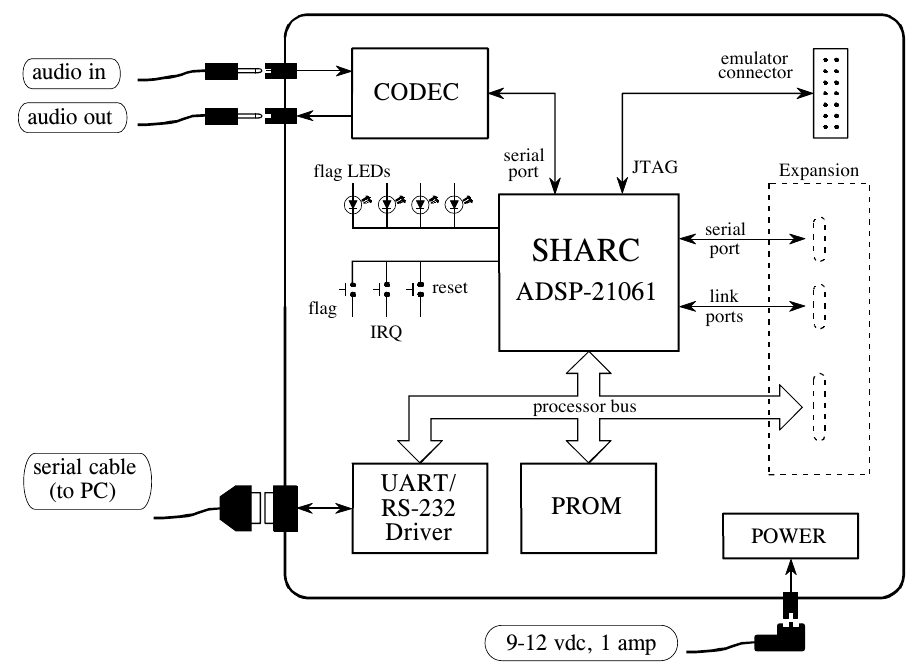
\includegraphics[width=0.767\linewidth,height=0.8\textheight,keepaspectratio]{assets/ch29/fig29-01.png}
\caption*{\textbf{图 29-1　EZ-KIT Lite 电路板的框图。}
只需要四个外部连接：音频输入、音频输出、连到个人计算机的串口（RS-232）线，以及电源。串口线和电源都随
EZ-KIT Lite 提供。 （audio in = 音频输入，audio out = 音频输出，CODEC =
编解码器，flag LEDs = 标志指示灯，flag = 标志按钮，IRQ =
中断请求按钮，reset = 复位按钮，serial port = 串口，JTAG = JTAG
接口，emulator connector = 仿真器接口，Expansion = 扩展区，link ports =
链路口，processor bus = 处理器总线，serial cable (to PC) = 串口线（连
PC），UART/RS-232 Driver = UART/RS-232 驱动器，PROM = 程序存储器，POWER
= 电源，9-12 vdc, 1 amp = 9～12 伏直流、1 安。）}
\end{figure}

模数转换和数模转换由一片 Analog Devices 的 AD1847 编解码器(codec，即
coder-decoder)完成。这是一个 16 位 Σ-Δ 转换器(sigma-delta
converter)，能以最高每秒 48k
个采样的速率数字化两个通道（立体声），同时以相同速率输出两个通道。由于这块板子主要用来处理音频信号，输入和输出是交流耦合的，截止频率约
20 Hz。

板上有三个按钮，分别用来产生中断、复位处理器，以及翻转一个系统可读的标志位。板上装有四个
LED，可以通过翻转位来点亮或熄灭。如果你有雄心，板上还有一些区域可以让你接触串口、链路口（只有用
ADSP-21062 的 EZ-LAB
才有）和处理器总线。不过这些位置是空的，你需要自己焊上接插件和其他元件。

它的工作方式是这样的：上电后，处理器从板上的 EPROM（512 k
字节）启动，装入一个程序，与你的个人计算机建立串行通信。接下来，你在 PC
上启动 EZ-Lite Host 程序，用它把程序下载到 DSP、把数据从 DSP
上传回来。EZ-KIT Lite
自带几个预先写好的程序，只要点击图标就能运行。例如，有一个带通程序，让你对着麦克风说话，听到经过带通滤波器后的结果。这些程序有两个用处：(1)
能让系统很快做出点有意思的事，让你相信它确实能用；(2)
为你编写自己的程序提供模板。这就引出了下一个话题：一个用 EZ-KIT Lite
的设计实例。

\section{设计实例：一个 FIR 音频滤波器}

把预先写好的程序摆弄一阵之后，你会想修改它们，积累编程经验。程序可以用汇编或
C 编写，EZ-KIT Lite
提供了支持这两种语言的软件工具。本章后面会介绍更高级的编程方法，比如仿真、调试和在集成开发环境中工作。眼下我们专注于让程序跑起来的最简单方法。小脚丫，迈小步。

\begin{figure}[htbp]
\centering
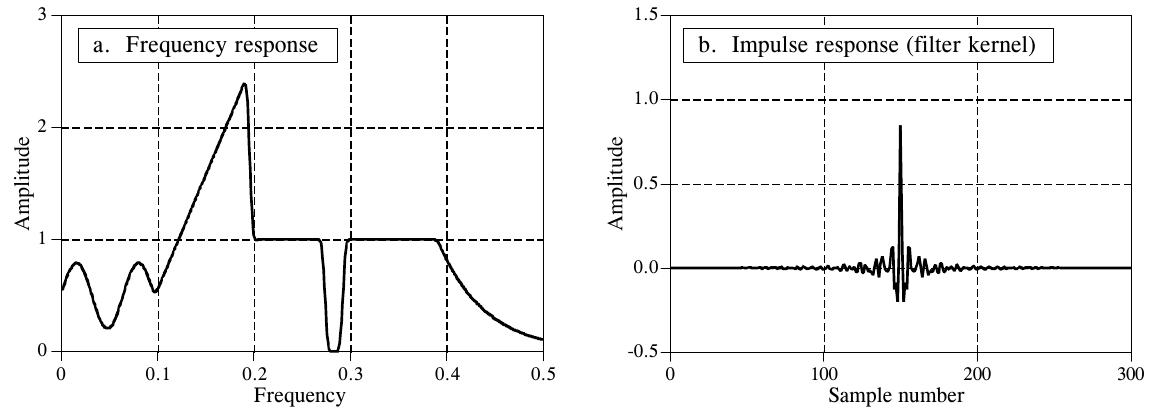
\includegraphics[width=0.958\linewidth,height=0.8\textheight,keepaspectratio]{assets/ch29/fig29-02.png}
\caption*{\textbf{图 29-2　FIR 滤波器实例。} (a)
是一个高度定制的滤波器的频率响应，(b)
是对应的冲激响应（滤波器核）。这个滤波器是在第 17 章设计的，用来说明 FIR
数字滤波器几乎可以实现任何频率响应。 （a. Frequency response =
频率响应；b. Impulse response (filter kernel) =
冲激响应（滤波器核）。Amplitude = 幅度，Frequency = 频率，Sample number
= 采样序号。）}
\end{figure}

由于源代码是 ASCII
文本，修改现有文件或编写全新的程序，只需要一个普通的文本编辑器。表 29-2
是一个用汇编编写的 FIR
滤波器程序的例子。虽然眼下你只需要关心这段代码，但要记住，构成一个完整的程序还需要其他文件。其中包括一个''体系结构描述文件''(architecture
description
file，定义硬件配置和存储器分配)、中断向量表的设置，以及编解码器的初始化例程。最终你得弄懂这些部分在做什么，但现在只需从预先写好的程序里把它们复制过来。

如表 29-2 开头所示，进入代码的主体之前，需要定义三个变量：滤波器核的点数
NR\_COEF；一个存放输入信号过去采样的循环缓冲区(circular buffer) dline{[}
{]}；一个存放滤波器核的循环缓冲区 coef{[}
{]}。我们还需要告诉程序另外两项信息：编解码器的采样率，以及包含滤波器核的文件名，以便把它读进
coef{[}
{]}。这些步骤都很简单，每一步不过一行代码。例子里没有列出它们，因为为了简单起见，它们放在我们略过的那些代码段里。

图 29-2 是我们用来测试这个程序的滤波器核，就是第 17
章设计的那个自定义滤波器。你应该还记得，这个滤波器特意选了一个非常不规则的频率响应，以强调
FIR 数字滤波器几乎可以实现你想要的任何频率响应。图 (a)
是测试滤波器的频率响应，(b) 是对应的冲激响应（即滤波器核）。这个 301
点的滤波器核存放在一个 ASCII
文件里，在链接时与其他代码段合在一起，形成一个可执行程序。

程序的主体做两件事。第 6～13
行配置数据地址发生器(data-address-generator，DAG)来管理两个循环缓冲区
dline{[} {]} 和 coef{[}
{]}。上一章讲过，每个缓冲区需要三个参数：缓冲区在存储器中的起始地址（b0
和 b8）、缓冲区的长度（l0 和 l8），以及缓冲区中数据的步长（m0 和
m8）。这些控制循环缓冲区的参数存放在 DAG
的硬件寄存器里，使它们能非常高效地访问和管理数据。

主程序的第二件事是一个''无所事事''的循环，在第 15～19
行。它什么也不做，只是等待一个表示输入采样已采集到的中断。这个程序的所有处理都是逐个采样(sample-by-sample)进行的：每从输入读入一个采样，就算出输出信号的一个采样并送往编解码器。大多数时域算法，比如
FIR 和 IIR
滤波器，都属于这一类。另一种方式是逐帧(frame-by-frame)处理，频域技术必须用这种方式。在逐帧处理中，先从输入读入一组采样，进行计算，再把一组采样写到输出。

响应''采样就绪''中断的子程序分为三段。第一段（第 27～33
行）以定点数的形式从编解码器取得采样，并把它转换为浮点数。在 SHARC
汇编语言中，数据寄存器存放定点数时记作 ``r''（如 r0、r8、r15
等），存放浮点数时记作 ``f''（如 f0、f8、f15）。例如第 32 行，数据寄存器
0 中的定点数（即 r0）被转换成浮点数，并覆盖数据寄存器 0（即
f0）。这次转换按数据寄存器 1（即
r1）中的定点数所指定的比例进行。第三段（第 47～53
行）执行相反的步骤：把输出采样的浮点数转换为定点数，送往编解码器。

把输入采样变成输出采样的 FIR 滤波器在第 35～45
行。所有计算都用浮点进行，因此不必操心缩放和溢出。如上一章所述，这段代码经过优化，利用了
SHARC DSP 每个时钟周期执行多条指令的能力。

\textbf{表 29-2　用汇编编写的 FIR 滤波器程序。}（注释已译成中文。）

进入主程序之前，必须先定义下面的常数和变量：

{\def\LTcaptype{none} % do not increment counter
\begin{longtable}[]{@{}ll@{}}
\toprule\noalign{}
名称 & 含义 \\
\midrule\noalign{}
\endhead
\bottomrule\noalign{}
\endlastfoot
NR\_COEF & 滤波器核的系数个数（本例为 301） \\
dline{[}NR\_COEF{]} & 存放过去输入采样的循环缓冲区，位于数据存储器 \\
coef{[}NR\_COEF{]} & 存放滤波器系数的循环缓冲区，位于程序存储器 \\
\end{longtable}
}

\begin{Shaded}
\begin{Highlighting}[]
\NormalTok{001     /************************************************************************}
\NormalTok{002     ******************      主程序                **********************}
\NormalTok{003     ************************************************************************/}
\NormalTok{004     main}\OperatorTok{:}
\NormalTok{005}
\NormalTok{006     /* 初始化 DAG，用来控制循环缓冲区 }\OperatorTok{*/}
\NormalTok{007}
\NormalTok{008     b0 }\OperatorTok{=}\NormalTok{ dline}\CommentTok{;        /* 设置 dline[ ]，存放过去输入采样的缓冲区 */}
\NormalTok{009     l0 }\OperatorTok{=} \FunctionTok{@}\ErrorTok{d}\NormalTok{line}\CommentTok{;}
\NormalTok{010     m0 }\OperatorTok{=} \DecValTok{1}\CommentTok{;}
\NormalTok{011     b8 }\OperatorTok{=}\NormalTok{ coef}\CommentTok{;         /* 设置 coef[ ]，存放滤波器系数的缓冲区 */}
\NormalTok{012     l8 }\OperatorTok{=} \FunctionTok{@}\ErrorTok{c}\NormalTok{oef}\CommentTok{;}
\NormalTok{013     m8 }\OperatorTok{=} \DecValTok{1}\CommentTok{;}
\NormalTok{014}
\NormalTok{015     /* 进入循环，等待"采样就绪"中断 */}
\NormalTok{016}
\NormalTok{017     }\BuiltInTok{wait}\OperatorTok{:}
\NormalTok{018     idle}\CommentTok{;}
\NormalTok{019     jump wait}\CommentTok{;}
\NormalTok{020}
\NormalTok{021}
\NormalTok{022     /***********************************************************************}
\NormalTok{023     *********     处理一个采样的子程序                     ***********}
\NormalTok{024     ***********************************************************************/}
\NormalTok{025     sample\_ready}\OperatorTok{:}
\NormalTok{026}
\NormalTok{027     /* 取得输入采样，转换为浮点数 */}
\NormalTok{028}
\NormalTok{029     r0 }\OperatorTok{=}\NormalTok{ dm}\OperatorTok{(}\NormalTok{rx\_buf }\OperatorTok{+} \DecValTok{1}\OperatorTok{)}\CommentTok{;           /* 把输入采样移入 r0 */}
\NormalTok{030     r0 }\OperatorTok{=}\NormalTok{ lshift r0 by }\DecValTok{16}\CommentTok{;          /* 移到最高 16 位，以保留符号 */}
\NormalTok{031     r1 }\OperatorTok{=} \OperatorTok{{-}}\DecValTok{31}\CommentTok{;                      /* 设置转换的比例 */}
\NormalTok{032     f0 }\OperatorTok{=}\NormalTok{ float r0 by r1}\CommentTok{;           /* 定点转浮点 */}
\NormalTok{033     dm}\OperatorTok{(}\NormalTok{i0}\OperatorTok{,}\NormalTok{m0}\OperatorTok{)} \OperatorTok{=}\NormalTok{ f0}\CommentTok{;                /* 把新采样存入 dline[ ]，并把 f12 清零 */}
\NormalTok{034}
\NormalTok{035     /* 用 FIR 滤波器计算输出采样 }\OperatorTok{*/}
\NormalTok{036}
\NormalTok{037     f12 }\OperatorTok{=} \DecValTok{0}\CommentTok{;                                         /* 预先装好寄存器 */}
\NormalTok{038     f2 }\OperatorTok{=}\NormalTok{ dm}\OperatorTok{(}\NormalTok{i0}\OperatorTok{,}\NormalTok{m0}\OperatorTok{),}\NormalTok{ f4 }\OperatorTok{=}\NormalTok{ pm}\OperatorTok{(}\NormalTok{i8}\OperatorTok{,}\NormalTok{m8}\OperatorTok{)}\CommentTok{;}
\NormalTok{039     f8 }\OperatorTok{=}\NormalTok{ f2}\OperatorTok{*}\NormalTok{f4}\OperatorTok{,}\NormalTok{ f2 }\OperatorTok{=}\NormalTok{ dm}\OperatorTok{(}\NormalTok{i0}\OperatorTok{,}\NormalTok{m0}\OperatorTok{),}\NormalTok{ f4 }\OperatorTok{=}\NormalTok{ pm}\OperatorTok{(}\NormalTok{i8}\OperatorTok{,}\NormalTok{m8}\OperatorTok{)}\CommentTok{;}
\NormalTok{040                                                    /* 高效的主循环 */}
\NormalTok{041     lcntr }\OperatorTok{=}\NormalTok{ NR\_COEF}\OperatorTok{{-}}\DecValTok{2}\OperatorTok{,}\NormalTok{ do }\OperatorTok{(}\NormalTok{pc}\OperatorTok{,}\DecValTok{1}\OperatorTok{)}\NormalTok{ until lce}\CommentTok{;}
\NormalTok{042     f8 }\OperatorTok{=}\NormalTok{ f2}\OperatorTok{*}\NormalTok{f4}\OperatorTok{,}\NormalTok{ f12 }\OperatorTok{=}\NormalTok{ f8}\OperatorTok{+}\NormalTok{f12}\OperatorTok{,}\NormalTok{ f2 }\OperatorTok{=}\NormalTok{ dm}\OperatorTok{(}\NormalTok{i0}\OperatorTok{,}\NormalTok{m0}\OperatorTok{),}\NormalTok{ f4 }\OperatorTok{=}\NormalTok{ pm}\OperatorTok{(}\NormalTok{i8}\OperatorTok{,}\NormalTok{m8}\OperatorTok{)}\CommentTok{;}
\NormalTok{043}
\NormalTok{044     f8 }\OperatorTok{=}\NormalTok{ f2}\OperatorTok{*}\NormalTok{f4}\OperatorTok{,}\NormalTok{ f12 }\OperatorTok{=}\NormalTok{ f8}\OperatorTok{+}\NormalTok{f12}\CommentTok{;                        /* 完成最后一轮循环 */}
\NormalTok{045     f12 }\OperatorTok{=}\NormalTok{ f8}\OperatorTok{+}\NormalTok{f12}\CommentTok{;}
\NormalTok{046}
\NormalTok{047     /* 把输出采样转换为定点数并输出 */}
\NormalTok{048}
\NormalTok{049     r1 }\OperatorTok{=} \DecValTok{31}\CommentTok{;                      /* 设置转换的比例 */}
\NormalTok{050     r8 }\OperatorTok{=}\NormalTok{ fix f12 by r1}\CommentTok{;           /* 浮点转定点 */}
\NormalTok{051     rti}\OperatorTok{(}\DataTypeTok{db}\OperatorTok{)}\CommentTok{;                      /* 从中断返回，但先执行接下来的 2 行 */}
\NormalTok{052     r8 }\OperatorTok{=}\NormalTok{ lshift }\KeywordTok{r8}\NormalTok{ by }\OperatorTok{{-}}\DecValTok{16}\CommentTok{;        /* 移到最低 16 位 */}
\NormalTok{053     dm}\OperatorTok{(}\NormalTok{tx\_buf }\OperatorTok{+} \DecValTok{1}\OperatorTok{)} \OperatorTok{=} \KeywordTok{r8}\CommentTok{;          /* 把采样送到输出 */}
\end{Highlighting}
\end{Shaded}

\begin{quote}
\textbf{译注：} 第 033 行的注释说''并把 f12
清零''，但这一行只是把新采样存进 dline{[} {]}，f12 实际是在第 037
行清零的。注释照原书翻译。
\end{quote}

写好汇编程序、设计好滤波器核之后，就可以生成能在 SHARC DSP
上执行的程序了。做法是依次运行编译器、汇编器和链接器，这三个程序都随
EZ-KIT Lite 提供。编译器把 C 程序转换成 SHARC
的汇编语言；如果像本例这样直接用汇编编写程序，就跳过这一步。汇编器和链接器把程序和外部文件（比如体系结构文件、编解码器初始化例程、滤波器核等）转换成最终的可执行文件。整个过程大约
30 秒，最终得到一个存放在你 PC 硬盘上的 SHARC 程序。然后用 EZ-KIT Lite
的主机程序在 EZ-KIT Lite 上运行它：只要点击你想让 DSP 运行的文件，EZ-KIT
Lite 主机程序就会处理其余的事，下载程序并启动运行。

这就引出了两个问题。第一，怎样测试我们的音频滤波器，确认它按设计在工作？第二，一家叫
Analog（模拟）Devices 的公司，到底为什么要做 Digital（数字）信号处理器？

\section{在 DSP 系统上做模拟测量}

暂时忘掉你正在学的是数字技术。让我们从一位专攻模拟电子学的工程师的角度来看这件事。他不关心
EZ-KIT Lite 里面是什么，只关心它有一个模拟输入和一个模拟输出。如图 29-3
所示，他会采用分析''黑盒子''的传统模拟方法：把信号发生器接到输入端，用示波器看输出。

\begin{figure}[htbp]
\centering
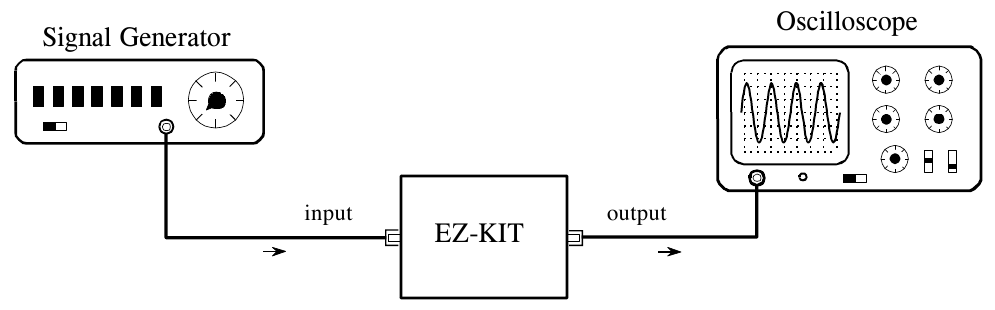
\includegraphics[width=0.829\linewidth,height=0.8\textheight,keepaspectratio]{assets/ch29/fig29-03.png}
\caption*{\textbf{图 29-3　测试 EZ-KIT Lite。}
模拟工程师测试一个系统的性能时，把信号发生器接到它的输入端，把示波器接到它的输出端。用这种方法测试一个
DSP 系统（比如 EZ-KIT Lite），它看起来就像一个近乎完美的模拟系统。
（Signal Generator = 信号发生器，Oscilloscope = 示波器，input =
输入，output = 输出。）}
\end{figure}

我们的模拟大师发现了什么？首先，系统是线性的（至少就这个简单测试所能判断的而言）。往输入端送一个正弦波，输出端看到的也是一个正弦波。改变输入的幅度或频率，输出也会相应变化。慢慢提高输入频率，到某一点时，输出正弦波的幅度会迅速降到零。这发生在略低于采样率一半的地方，是
ADC 上抗混叠滤波器(anti-alias filter)作用的结果。

接着，我们的工程师注意到了模拟世界里没有的东西：这个系统具有完美的线性相位。换句话说，输入信号中发生一个事件，与这个事件在输出信号中产生结果之间，有一个恒定的延迟。例如，考虑我们的示例滤波器核（图
29-2）。由于它的对称中心在第 150 个采样，输出信号相对于输入信号会延迟
150 个采样。例如，如果系统以 8 kHz 采样，这个延迟就是 18.75
毫秒。此外，Σ-Δ 转换器还会额外带来一小段固定延迟。

\begin{quote}
\textbf{译注：} 原书这里写的是''图 29-3 中的示例滤波器核''，但图 29-3
是测试接线图，滤波器核在图 29-2，译文已改正。
\end{quote}

我们的模拟工程师看到这种线性相位会非常焦躁。信号看起来不像他以为的样子，他会开始飞快地拧旋钮。他会抱怨触发不正常，嘴里嘀咕着''这说不通啊''、``怎么回事？''、``谁动过我的示波器？''之类的话。DSP
系统的性能好到这种程度，他得花上几分钟才能明白自己看到的是什么。

为了让他更加佩服，我们请这位工程师手动测量系统的频率响应。为此，他把信号发生器从
125 Hz 到 10 kHz、以 125 Hz
为步长逐一调过每个频率。在每个频率上，他测出输出信号的幅度，再除以输入信号的幅度。（当然，最省事的做法是让输入信号保持恒定幅度。）这次测试我们把
EZ-KIT Lite 的采样率设为 22 kHz。也就是说，图 29-2a 中 0～0.5
的数字频率，对应真实测量中的直流到 11 kHz。

\begin{figure}[htbp]
\centering
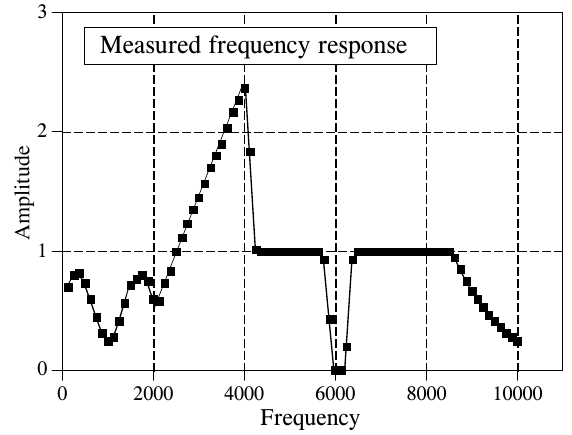
\includegraphics[width=0.477\linewidth,height=0.8\textheight,keepaspectratio]{assets/ch29/fig29-04.png}
\caption*{\textbf{图 29-4　实测的频率响应。} 这张图是示例 FIR
滤波器频率响应上的实测点。这些实测点的精度远不如图 29-2a
中设计的频率响应。 （Measured frequency response =
实测的频率响应，Amplitude = 幅度，Frequency =
频率（Hz）。原书图注写的是''图 29-3a''，应为图 29-2a。）}
\end{figure}

图 29-4 是在 EZ-KIT Lite
上实际测得的数据，好得不能再好了！实测数据点在测量误差范围内与理论曲线吻合。这是我们的模拟工程师用电阻、电容和电感做的滤波器从未见过的。

不过，即便如此，也还没给 DSP
应得的评价。用示波器和数字电压表做的模拟测量，典型的准确度和精密度约为
0.1\%～1\%。相比之下，这个 DSP 系统只受 16 位编解码器约 0.001\%
的舍入误差限制，因为内部计算用的是浮点。换句话说，被测器件比所用的测量工具精确一百倍。要正确评估这个频率响应，需要专门的仪器，比如带
20 位 ADC 的计算机化数据采集系统。考虑到这些事实，DSP
常被用在测量仪器中以获得高精度，也就不足为奇了。

现在可以回答这个问题了：Analog Devices
为什么要卖数字信号处理器？仅仅十年前，最先进的信号处理还是用精密运放和类似的晶体管电路来完成的。而今天，最高品质的模拟处理是用数字技术实现的。Analog
Devices
是个人和其他公司的好榜样：坚持你的愿景和目标，但不要害怕随着技术的变化而调整！

\section{再看定点与浮点}

在上一个例子中，我们利用了 SHARC DSP
的一个关键特性：处理浮点运算的能力。尽管采样在送入和送出编解码器时是定点格式，我们还是不嫌麻烦地把它们转换成浮点数，用于中间的
FIR
滤波算法。上一章讲过，用浮点数学处理数据有两个理由：编程方便和性能好。这真的有区别吗？

对程序员来说，有，而且区别很大。浮点代码要好写得多。回头看看表 29-2
的汇编程序，FIR 滤波器的主体只有两行（第 41 和 42
行）。相比之下，定点程序员必须在每一步数学运算处都加上管理数据的代码。为了避免上溢和下溢，必须检查数值的大小，必要时做相应的缩放。中间结果还需要存放在扩展精度的累加器中，以免反复的舍入误差造成灾难性的后果。

性能问题要微妙得多。例如，图 29-5a 是一个截止较陡的 FIR
低通滤波器，就是第 16
章讲的那种。这条''大尺度''的曲线，不论计算时用定点还是浮点，看起来都一样。要看出两种方法的区别，必须像
(b)、(c)、(d)
那样把幅度放大几百倍。这时就能看到明显的差别了。浮点执行的结果 (b)
舍入噪声非常低，以至于它的性能受限于我们设计滤波器核的方式。过渡带附近
0.02\% 的过冲，是这个滤波器所用布莱克曼窗(Blackman
window)的特征。重点是，如果想提高性能，我们需要改进的是算法，而不是实现。(c)
和 (d) 的曲线显示了滤波器核的每个点分别用 16 位和 14
位表示时引入的舍入噪声。再好的算法也无法让这两条曲线变好，实际频率响应的形状已经被噪声淹没了。

\begin{figure}[htbp]
\centering
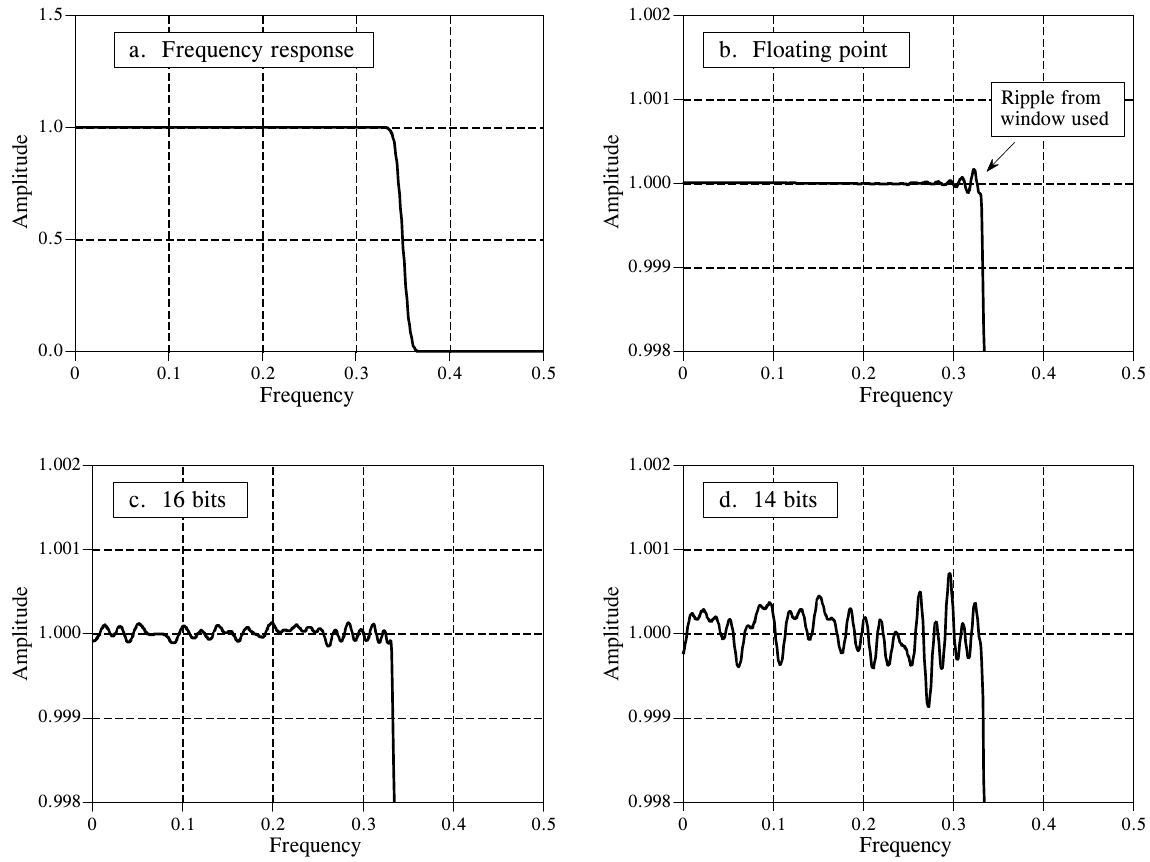
\includegraphics[width=0.958\linewidth,height=0.8\textheight,keepaspectratio]{assets/ch29/fig29-05.png}
\caption*{\textbf{图 29-5　频率响应中的舍入噪声。} (a) 是一个加窗 sinc
低通滤波器的频率响应，使用布莱克曼窗，滤波器核有 150 个点。(b)、(c)、(d)
把幅度放大，更细地显示这个响应。当滤波器核用浮点表示时
(b)，舍入噪声与加窗 sinc 设计本身的不完美相比微不足道。如 (c) 和 (d)
所示，用定点表示滤波器核，舍入噪声就成了主要的缺陷。 （a. Frequency
response = 频率响应；b. Floating point = 浮点；c.~16 bits = 16 位；d.~14
bits = 14 位；Ripple from window used = 所用窗函数造成的纹波。Amplitude
= 幅度，Frequency = 频率。）}
\end{figure}

图 29-6 显示了定点和浮点在时域中的区别。图 (a)
是一个幅度按指数衰减的振荡信号。它可以代表比如拨弦的声波，或远处爆炸引起的地面震动。和前面一样，这个''大尺度''的波形，不论用定点还是浮点表示采样，看起来都一样。要看出区别，必须像
(b)、(c)、(d) 那样把幅度放大。第 3
章讲过，这种量化表现得很像加性随机噪声，限制了信号中微小成分的可检测性。

\begin{figure}[htbp]
\centering
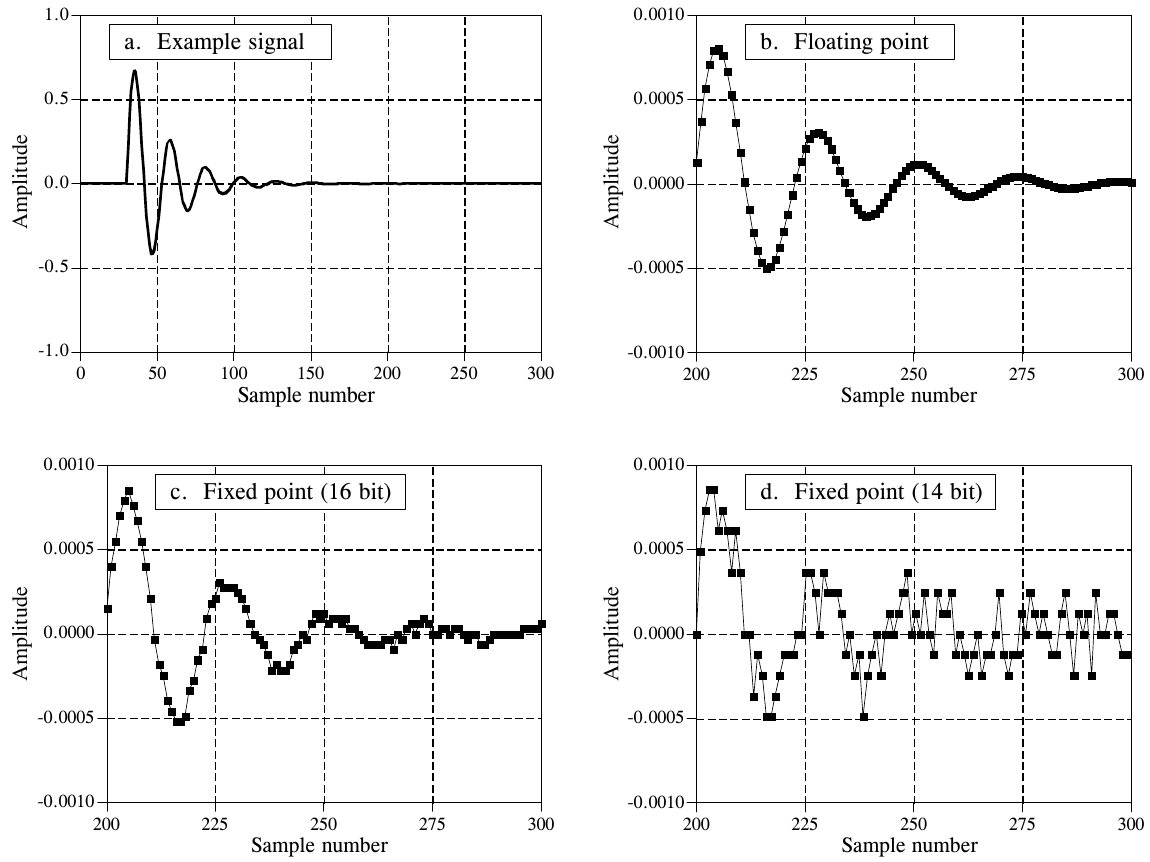
\includegraphics[width=0.958\linewidth,height=0.8\textheight,keepaspectratio]{assets/ch29/fig29-06.png}
\caption*{\textbf{图 29-6　时域中的舍入噪声。} (a)
是一个幅度按指数衰减的示例信号。(b)、(c)、(d)
把幅度放大，更细地显示它。信号用浮点表示时
(b)，舍入噪声低到在这张图中根本看不出来。如 (c) 和 (d)
所示，用定点表示信号，产生的舍入噪声要高得多。 （a. Example signal =
示例信号；b. Floating point = 浮点；c.~Fixed point (16 bit) = 定点（16
位）；d.~Fixed point (14 bit) = 定点（14 位）。Amplitude = 幅度，Sample
number = 采样序号。）}
\end{figure}

定点和浮点之间的这些性能差别，很多时候并不重要；例如，在图 29-5a 和图
29-6a
这样的''大尺度''信号中甚至看不出来。不过，在有些应用中，浮点额外的性能是有帮助的，甚至可能至关重要。例如，高保真的消费级音频系统（比如
CD 播放机）用 16
位定点表示信号。大多数情况下，这已经超出了人耳的能力。然而，最好的专业音频系统以高达
20～24
位对信号采样，绝不给可能污染音乐的伪影留任何余地。浮点几乎是处理这类高精度数字信号的算法的理想选择。

另一种需要浮点更高性能的情形，是算法对噪声特别敏感的时候。例如，FIR
滤波器对舍入效应相当不敏感。如图 29-5
所示，舍入噪声不会改变频率响应的整体形状，整条曲线只是变得更''毛''一些。IIR
滤波器就是另一回事了：舍入可能造成各种破坏，包括让滤波器变得不稳定。浮点使这些算法在截止频率的陡峭程度、阻带衰减和阶跃响应过冲方面都能取得更好的性能。

\section{高级软件工具}

我们的自定义滤波器例子展示了让程序在 SHARC DSP
上运行的最简单方法：编辑、汇编、链接、下载，每一步由单独的程序完成。这种方法对简单任务来说没有问题，但对高级程序员，还有更好的软件工具。我们来看看当你真正认真对待
DSP 时，有哪些工具可用。

我们要考察的第一个工具是 C 编译器。上一章讲过，汇编和 C 都常用于 DSP
编程。使用 C 的一个巨大优势是函数库，既有标准 C 操作，也有 DSP 算法。表
29-3 列出了 SHARC DSP 的部分 C 库函数。数学类函数包括许多 DSP
中常用的函数，比如三角函数（sin、cos、tan
等）、对数和指数。如果你的程序需要这类函数，单凭这一点大概就足以让你选择
C 而不是汇编了。要特别留意表 29-3 中''信号处理''类的例程，那里有关键的
DSP 算法，包括实数和复数 FFT、FIR 和 IIR
滤波器，以及均值、均方根值和方差等统计函数。当然，这些例程都是用汇编编写的，因此在速度和存储器占用上都非常高效。

\textbf{表 29-3　C 库函数。} 这是用 C 为 Analog Devices SHARC DSP
编程时可用函数的部分列表。

\textbf{数学运算(MATH OPERATIONS)}

{\def\LTcaptype{none} % do not increment counter
\begin{longtable}[]{@{}llll@{}}
\toprule\noalign{}
函数 & 功能 & 函数 & 功能 \\
\midrule\noalign{}
\endhead
\bottomrule\noalign{}
\endlastfoot
abs & 绝对值 & fmod & 取模 \\
acos & 反余弦 & log & 自然对数 \\
asin & 反正弦 & log10 & 以 10 为底的对数 \\
atan & 反正切 & matadd & 矩阵加法 \\
atan2 & 商的反正切 & matmul & 矩阵乘法 \\
cabsf & 复数绝对值 & pow & 乘方 \\
cexpf & 复指数 & rand & 随机数发生器 \\
cos & 余弦 & sin & 正弦 \\
cosh & 双曲余弦 & sinh & 双曲正弦 \\
cot & 余切 & sqrt & 平方根 \\
div & 除法 & srand & 随机数种子 \\
exp & 指数 & tan & 正切 \\
& & tanh & 双曲正切 \\
\end{longtable}
}

\textbf{字符与字符串处理(CHARACTER \& STRING MANIPULATION)}

{\def\LTcaptype{none} % do not increment counter
\begin{longtable}[]{@{}llll@{}}
\toprule\noalign{}
函数 & 功能 & 函数 & 功能 \\
\midrule\noalign{}
\endhead
\bottomrule\noalign{}
\endlastfoot
atoi & 字符串转整数 & memchr & 查找字符的第一次出现 \\
bsearch & 数组二分查找 & memcpy & 复制字符 \\
isalnum & 检测字母或数字字符 & strcat & 连接字符串 \\
isalpha & 检测字母字符 & strcmp & 比较字符串 \\
iscntrl & 检测控制字符 & strerror & 取错误信息 \\
isdigit & 检测十进制数字 & strlen & 字符串长度 \\
isgraph & 检测可打印字符 & strncmp & 比较若干字符 \\
islower & 检测小写字符 & strrchr & 查找字符的最后一次出现 \\
isprint & 检测可打印字符 & strstr & 在字符串中查找子串 \\
ispunct & 检测标点字符 & strtok & 把字符串拆分为记号 \\
isspace & 检测空白字符 & system & 把字符串发给操作系统 \\
isupper & 检测大写字符 & tolower & 大写转小写 \\
isxdigit & 检测十六进制数字 & toupper & 小写转大写 \\
\end{longtable}
}

\textbf{程序控制(PROGRAM CONTROL)}

{\def\LTcaptype{none} % do not increment counter
\begin{longtable}[]{@{}ll@{}}
\toprule\noalign{}
函数 & 功能 \\
\midrule\noalign{}
\endhead
\bottomrule\noalign{}
\endlastfoot
abort & 异常终止程序 \\
calloc & 分配并初始化存储器 \\
free & 释放存储器 \\
idle & 处理器空闲指令 \\
interrupt & 定义中断处理 \\
poll\_flag\_in & 测试输入标志 \\
set\_flag & 设置处理器标志 \\
timer\_off & 关闭处理器定时器 \\
timer\_on & 打开处理器定时器 \\
timer\_set & 初始化处理器定时器 \\
\end{longtable}
}

\textbf{信号处理(SIGNAL PROCESSING)}

{\def\LTcaptype{none} % do not increment counter
\begin{longtable}[]{@{}ll@{}}
\toprule\noalign{}
函数 & 功能 \\
\midrule\noalign{}
\endhead
\bottomrule\noalign{}
\endlastfoot
a\_compress & A 律压缩 \\
a\_expand & A 律扩展 \\
autocorr & 自相关 \\
biquad & 双二阶(biquad)滤波器节 \\
cfftN & 复数 FFT \\
crosscorr & 互相关 \\
fir & FIR 滤波器 \\
histogram & 直方图 \\
iffN & 复数逆 FFT \\
iir & IIR 滤波器 \\
mean & 数组的均值 \\
mu\_compress & μ 律压缩 \\
mu\_expand & μ 律扩展 \\
rfftN & 实数 FFT \\
rms & 数组的均方根值 \\
\end{longtable}
}

\begin{quote}
\textbf{译注：} 原书把逆 FFT 函数印成
\texttt{iffN}，按命名规律（cfftN、rfftN）应为 \texttt{ifftN}；system
的说明 ``sent string'' 应为 ``send
string''。函数名照原书保留。正文还提到''方差''，但表中列出的统计函数只有
mean 和 rms，因为这只是部分列表。
\end{quote}

表 29-4 是一个 C 程序的例子，取自 Analog Devices 的《C
编译器指南与参考手册》(C Compiler Guide and Reference
Manual)。这个程序通过把信号的延迟版本加到它自身上来产生回声。输入信号最近的
4000
个采样存放在一个循环缓冲区中。每采集到一个采样，就更新循环缓冲区，把最新的采样与最旧采样的一个缩放版本相加，并把结果送到输出。

\textbf{表 29-4}（原书只有表号，没有表题；注释已译成中文。这是 SHARC
专用的 C，依赖 \texttt{21020.h}、\texttt{macros.h} 等厂商头文件，不能在
PC 上编译。）

\begin{Shaded}
\begin{Highlighting}[]
\CommentTok{/*    CIRCBUF.C                                                              */}
\CommentTok{/*    这是为 ADSP{-}21061 EZ{-}KIT Lite 用 C 编写的回声程序。回声程序在直通(talkthru)  */}
\CommentTok{/*    程序的基础上加了一个循环缓冲机制。                                      */}
\CommentTok{/*    循环缓冲区由函数 CIRCULAR\_BUFFER、BASE 和 LENGTH 定义。回声是把当前输入   */}
\CommentTok{/*    加到最旧的输入上产生的。改变 BUFF\_LENGTH 就能修改回声的延迟。             */}
\CommentTok{/*                                                                           */}
\PreprocessorTok{\#include }\ImportTok{\textless{}21020.h\textgreater{}}\PreprocessorTok{           }\CommentTok{/* 为了 idle() 命令 */}
\PreprocessorTok{\#include }\ImportTok{\textless{}signal.h\textgreater{}}\PreprocessorTok{          }\CommentTok{/* 为了 interrupt 命令 */}
\PreprocessorTok{\#include }\ImportTok{\textless{}macros.h\textgreater{}}\PreprocessorTok{          }\CommentTok{/* 为了 CIRCULAR\_BUFFER 和 segment 函数 */}

\PreprocessorTok{\#define BUFF\_LENGTH }\DecValTok{4000}
                                                     \CommentTok{/* 把 echo 定义为 21k 的 DAG1 寄存器 i1 */}
\NormalTok{CIRCULAR\_BUFFER }\OperatorTok{(}\DataTypeTok{float}\OperatorTok{,}\DecValTok{1}\OperatorTok{,}\NormalTok{echo}\OperatorTok{)}                       \CommentTok{/* 指向循环缓冲区的一个 DM 指针 */}

\DataTypeTok{volatile} \DataTypeTok{float}\NormalTok{ in\_port segment }\OperatorTok{(}\NormalTok{hip\_reg0}\OperatorTok{);}           \CommentTok{/* hip\_reg0 和 hip{-}reg2 */}
\DataTypeTok{volatile} \DataTypeTok{float}\NormalTok{ out\_port segment }\OperatorTok{(}\NormalTok{hip\_reg2}\OperatorTok{);}          \CommentTok{/* 在体系结构文件中使用 */}

\DataTypeTok{void}\NormalTok{ process\_input }\OperatorTok{(}\DataTypeTok{int}\OperatorTok{);}
\DataTypeTok{void}\NormalTok{ main }\OperatorTok{(}\DataTypeTok{void}\OperatorTok{)}

\OperatorTok{\{}       \CommentTok{/* 把它做成变长数组。如果仿真器停在 main 处，而 dm 窗口里的              */}
        \CommentTok{/* \_BUFF\_LENGTH 被修改了，回声延迟也随之改变。                          */}
        \CommentTok{/* BUFF\_LENGTH 不要大于栈的大小！                                      */}

\DataTypeTok{float}\NormalTok{ data\_buff }\OperatorTok{[}\NormalTok{BUFF\_LENGTH}\OperatorTok{];}
\NormalTok{interrupt }\OperatorTok{(}\NormalTok{SIG\_IRQ3}\OperatorTok{,}\NormalTok{ process\_input}\OperatorTok{);}

\NormalTok{BASE }\OperatorTok{(}\NormalTok{echo}\OperatorTok{)} \OperatorTok{=}\NormalTok{ data\_buff}\OperatorTok{;}                          \CommentTok{/* 用缓冲区起始地址装入 b1 和 i1 */}
\NormalTok{LENGTH }\OperatorTok{(}\NormalTok{echo}\OperatorTok{)} \OperatorTok{=}\NormalTok{ BUFF\_LENGTH}\OperatorTok{;}                      \CommentTok{/* 用缓冲区长度装入 L1 */}

        \CommentTok{/* 数组填满后，第 n 个位置存放最新的值，第 n+1 个位置存放最旧的值。 */}

\ControlFlowTok{while} \OperatorTok{(}\DecValTok{1}\OperatorTok{)}
 \OperatorTok{\{}                                                \CommentTok{/* 回声输出最新值与 */}
  \DataTypeTok{float}\NormalTok{ oldest}\OperatorTok{,}\NormalTok{ newest}\OperatorTok{;}                           \CommentTok{/* 最旧值之和 */}
\NormalTok{  idle}\OperatorTok{();}

       \CommentTok{/* 中断例程返回后，echo 指向第 n 个位置。把新值放进变量 \textquotesingle{}newest\textquotesingle{}。 */}
       \CommentTok{/* 访问之后把指针加一，指向第 n+1 个位置。                         */}
\NormalTok{    CIRC\_READ }\OperatorTok{(}\NormalTok{echo}\OperatorTok{,} \DecValTok{1}\NormalTok{ newest}\OperatorTok{,}\NormalTok{ dm}\OperatorTok{);}

       \CommentTok{/* 现在 echo 指向 n+1。读出这个位置的值放进变量 \textquotesingle{}oldest\textquotesingle{}。          */}
       \CommentTok{/* 不更新指针，因为它现在正指向中断处理程序要写入的新位置。         */}
\NormalTok{    CIR\_READ }\OperatorTok{(}\NormalTok{echo}\OperatorTok{,} \DecValTok{0}\OperatorTok{,}\NormalTok{ oldest}\OperatorTok{,}\NormalTok{ dm}\OperatorTok{);}

         \CommentTok{/* 把最旧值和最新值相加，从端口送出 */}
\NormalTok{     out\_port}\OperatorTok{=}\NormalTok{oldest}\OperatorTok{+}\NormalTok{newest}\OperatorTok{;}
    \OperatorTok{\}}
\OperatorTok{\}}

\DataTypeTok{void}\NormalTok{ process\_input }\OperatorTok{(}\DataTypeTok{int}\NormalTok{ int\_number}\OperatorTok{)}
\OperatorTok{\{}
      \CommentTok{/* 最新的输入值写在第 n 个位置上、覆盖最旧的值，指针不更新。 */}
\NormalTok{  CIRC\_WRITE }\OperatorTok{(}\NormalTok{echo}\OperatorTok{,} \DecValTok{0}\OperatorTok{,}\NormalTok{ in\_port}\OperatorTok{,}\NormalTok{ dm}\OperatorTok{);}
\OperatorTok{\}}
\end{Highlighting}
\end{Shaded}

\begin{quote}
\textbf{译注：}
原书这段程序有几处排印问题：\texttt{CIRC\_READ\ (echo,\ 1\ newest,\ dm)}
在 \texttt{1} 后漏了逗号；\texttt{CIR\_READ} 应为
\texttt{CIRC\_READ}。另外，正文说''把最新采样与最旧采样的一个\textbf{缩放}版本相加''，但程序里是
\texttt{oldest+newest}，并没有缩放。代码照原书保留。
\end{quote}

下一个你应该寻找的高级软件工具，是集成开发环境(integrated development
environment，IDE)。这个时髦的术语，意思是编程和测试 DSP
所需的一切都整合进一个运转顺畅的软件包里。Analog Devices 在一个叫
VisualDSP® 的产品中提供了集成开发环境，运行在 Windows® 95 和 Windows NT™
下。图 29-7
是它主界面的一个例子，提供了一种无缝地编辑、构建和调试程序的方式。

\begin{figure}[htbp]
\centering
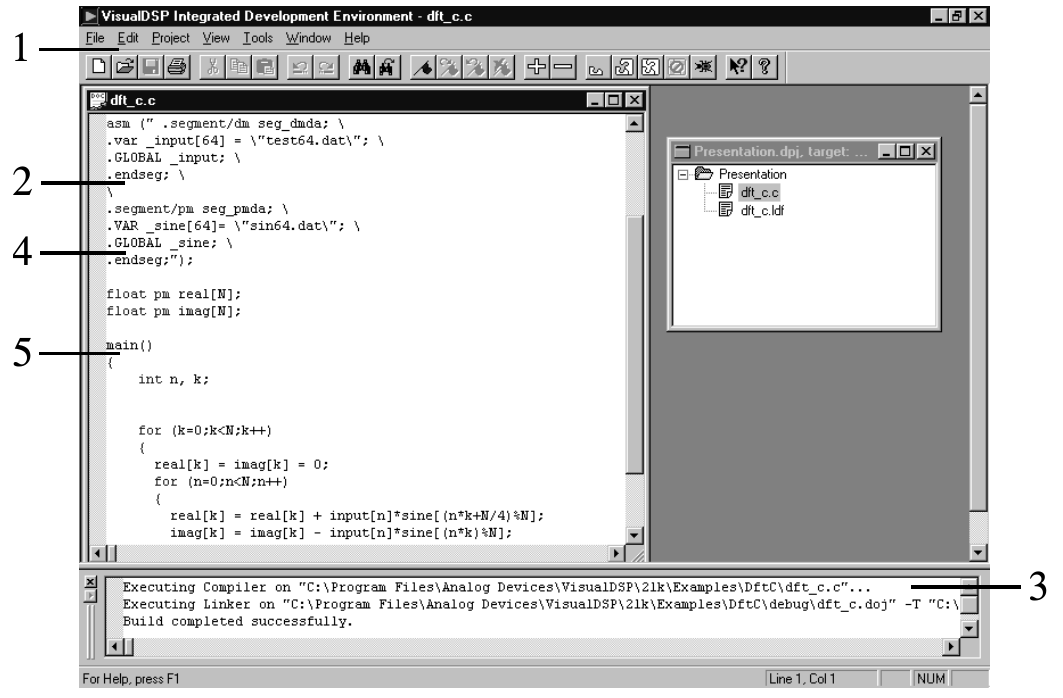
\includegraphics[width=0.886\linewidth,height=0.8\textheight,keepaspectratio]{assets/ch29/fig29-07.png}
\caption*{\textbf{图 29-7　VisualDSP 的示例界面。} 它为在 SHARC
上开发程序提供了一个集成开发环境。下列功能都可以从这一个界面访问：编辑、编译、汇编、链接、仿真、调试、下载和生成
PROM。图中编号标出的功能： 1. 在编辑、构建和调试之间轻松切换 2.
在同一个源文件里混用汇编和 C 3. 查看''构建''结果 4. 理解语法的强大编辑器
5. 通过书签轻松访问}
\end{figure}

（原书把这五条说明列在截图下方，裁图时已去掉，译文见上。）

下面是 VisualDSP
的一些关键特性，说明了集成开发环境为什么对快速软件开发如此重要。它的编辑器专门用来编写
C、汇编以及两者混合的程序。例如，它理解这些语言的语法，能用不同颜色显示不同类型的语句。你还可以同时编辑多个文件。这非常方便，因为最终的程序是由几个文件链接在一起生成的。

\begin{figure}[htbp]
\centering
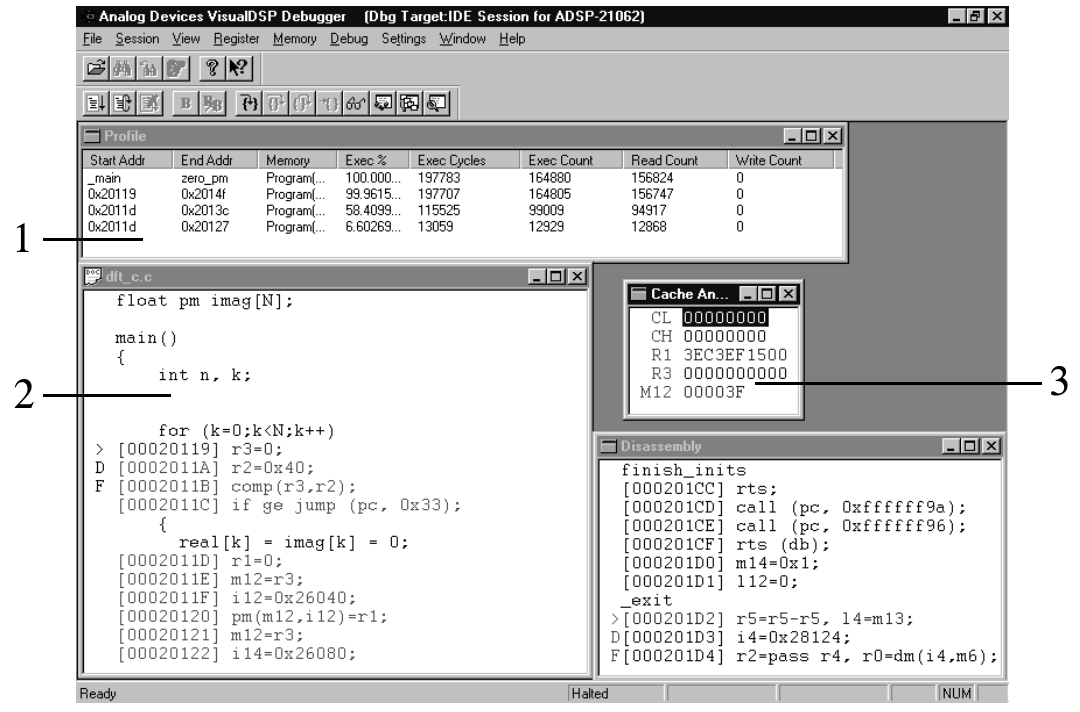
\includegraphics[width=0.900\linewidth,height=0.8\textheight,keepaspectratio]{assets/ch29/fig29-08.png}
\caption*{\textbf{图 29-8　VisualDSP 的调试界面。}
这是仿真和硬件仿真共用的界面。它可以查看穿插着对应汇编代码的 C
程序，跟踪指令的执行，检查寄存器（硬件寄存器、软件寄存器和存储器），跟踪总线活动，以及完成许多其他任务。图中编号标出的功能：
1. 剖析(profile)代码，找出瓶颈 2. 查看 C 与汇编的混合列表 3.
创建自定义的寄存器窗口}
\end{figure}

（原书把这三条说明列在截图下方，裁图时已去掉，译文见上。）

图 29-8 是 VisualDSP
调试器的一个示例界面。它是两类不同工具的接口：软件仿真器(simulator)和硬件仿真器(emulator)。软件仿真器在个人计算机里测试代码，甚至不需要有
DSP。这通常是程序写好后的第一步调试。软件仿真器模拟硬件的体系结构和运行，包括输入数据流、中断和其他
I/O。硬件仿真器（比如 Analog Devices 的
EZ-ICE®）在实际硬件上检查程序的运行。这要求硬件仿真软件（在你的 PC
上）能够监视 DSP 内部的电信号。为此，SHARC DSP 配有 IEEE 1149.1 JTAG
测试访问端口(Test Access Port)，让外部设备能够跟踪处理器的内部功能。

\begin{quote}
\textbf{译注：} 原书写作 ``IEEE 1140.1''，JTAG 标准的编号是 IEEE
1149.1，译文已改正。
\end{quote}

用过评估套件、考虑过购买高级软件工具之后，你还应该考虑参加培训班。许多
DSP 厂商都开设这类课程。例如，Analog Devices 提供为期 3
天的课程，每年在几个不同地点开课数次。这是向专家学习 DSP
的好途径。详情请查看厂商的网站。
